\chapter{Introduction}
\label{chap:introduction}
\tightlists


\subsection{Notes}
- thesis is split into two sections, noise in a single reporter affecting phenotype and how is noise specified across different genes.
- talk about Arjun's cancer papers
- talk about sui huang papers


CAS chapter - - sources of noise
- include Roy Wollman's paper for the CAS chapter. 
    - Says that the cell-state explains most of the variance. Things like volume, differntiation state, cell cycle, amount and timing of Ca+2 activation.
Variability and memory of protein levels in human cells - this argues that genes in the same pathway share variability.


    



Over the past few decades we have made huge advances in sequencing genomes. We now have  comprehensive catalogs of common and rare variation in humans and a few other species. These results have encouraged pursuits in synthetic biology and precision medicine. However, these pursuits have exposed the reality that we are still limited in our understanding of how genomic sequences reliably specify function. 

We now know that genetically identical cells grown in the same environment express different amounts of the same gene. Cell-to-cell variability has been shown to be functionally important. For example, individual cells in a population of stem cells differ in their differentiation potential \cite{chang_transcriptome-wide_2008}. When cells with the same genotype behave differently, this limits our ability to design drugs to target diseased cells and hinders our ability to design synthetic biological circuits that perform reliably over a period of time \cite{elowitz_synthetic_2000}. In order to understand biological systems, we need to understand the sources and extent of this cell-to-cell variability.

Work done in the previous decade using two copy reporters in E. Coli \cite{elowitz_stochastic_2002} and Yeast \cite{raser_control_2004} showed that cell-to-cell variability of gene expression is prevalent. To date, most of the work in understanding cell-to-cell variability has been done using reporters attached to a single gene or a few genes. How much of the variability at one locus is shared across different genes in the genome is still not well understood. I will address this question in *Aim 1*.



\subsection{Background}

\subsection{Gene expression variability exists amongst cells}

Gene expression is the result of probabilistic interactions between molecules in the cell. These molecules include the two copies of DNA, transcription factors, RNA polymerase amongst others. The low numbers of molecules involved in transcription results in  variable gene expression across cells and time. It is still a mystery how in the presence of these gene expression fluctuations biological systems function in an orderly manner.

The phenomenon of variability between cells is not new. Novick and Weiner \cite{novick_enzyme_1957} \cite{raj_nature_2008} described a phenonmenon in 1957 where given a population of E. Coli, the fraction of cells that produce beta galactidase is not deterministic. This fraction is stochastic and varies with the concentration of the inducer. The increase in the concentration of inducer only increases the chance that a bacterium produces beta galactidase. Given a fixed concentration of the inducer, it is not possible to predict with certainty if a single bacterium will produce beta galactidase but it is possible to estimate the probability of this event.

In 2002, Elowitz et al.  \cite{elowitz_stochastic_2002} showed using two-colored reporters in E. Coli that identical genes on two different chromosomes show cell-to-cell variability in expression. The authors decomposed this variability into two components. The first is intrinsic noise that is specific to a locus. Intrinsic noise is due to the local interactions of molecules involved in transcription at a locus. These might include promoters switching between active and inactive states, proteins binding to enhancers, recruitment of RNA polymerase and so on. The second source of variability is extrinsic noise. Extrinsic noise is due to differences between cells in the cellular milieu. The cellular milieu can include upstream regulators of transcription such as transcription factor concentrations, number of ribosomes in the cell etc. These differences in the cellular environment is likely to affect the expression of multiple genes. Follow-up studies have now confirmed the observation that genetically identical cells in the same environment display variability in gene expression \cite{raser_control_2004,blake_phenotypic_2006,blake_noise_2003,raser_noise_2005,volfson_origins_2006}.

- need more paragraphs here
- talk about arjun's fish work
- talk about rob singer
- talk about Dan larson
- talk about Ido golding


\subsection{Cell-to-Cell variability can result in functional differences}
An increase in cell-to-cell variability in gene expression has been observed in cells undergoing differentiation. Richard et al.  \cite{richard_single-cell-based_2016} looked at a well-studied differentiation system of chicken erythroid progenitors differentiating into erythrocytes. The authors showed that chicken erythroid cells show an increase in variability of gene expression of relevant genes prior to differentiation. Similar results were obtained by Mojtahedi et al  \cite{mojtahedi_cell_2016} while studying the differentiation of murine heamatopoetic progenitor cells into myeloid or erythroid cells. The authors hypothesize that this surge in variability allows the cells to transition out of stable cell-states and transition to different cell-states. 


Other examples have shown that genetically identical cells don't all reprogram at the same rate. Hanna and Saha et al. showed that reprogramming of somatic cells to iPSCs is stochastic with a random subset of initial cells completing reprogramming  \cite{hanna_direct_2009}. The authors showed that eventually all somatic cells reprogram to pluripotent stem cells when induced with transcription factors but the rate at which cells reprogram can be increased by increasing the cell-division rate. Similar stochasticity has been observed when fibroblasts were reprogrammed into induced endoderm progenitor cells \cite{biddy_single-cell_2018}.

Variability in phenotype has also been shown to be functionally important at the organismal level. In C. elegans, two identical cells from different lineages known as alpha cells always give rise to exactly one ventral uterine progenitor cell and one anchor cell \cite{seydoux_cell_1989}. Both the alpha cells have the potential to generate either of the two downstream cell-types but the cell fate is decided in a stochastic and co-ordinated manner. This case is a well-studied model of a stochastic cell-fate decision where a robust outcome is produced as a result of a stochastic choice. In another example in C. elegans, mutations that cause incomplete penetrance have been shown to be due to increased variability in the expression of cell-fate determining genes  \cite{raj_variability_2010}.  The mutants display increased variability in the expression of a gene called *end-1*. Cells with high-levels of *end-1* are able to activate downstream targets in the intestinal fate specification network whereas the cells with low levels of *end-1* do not. 

In bacteria, individual bacterium often display a persistor phenotype and grow at slower rates by expressing different subsets of genes. This confers the bacteria an ability to survive adverse changes such as antibiotic treatment that might otherwise terminate a homogenous population \cite{veening_bet-hedging_2008}. In yeast, variability has been observed in the utilization of the sugar galactose. The Gal genes that are responsible for the metabolism of galactose pathway display a bimodal expression pattern \cite{acar_enhancement_2005}. This bimodality has been explained using stochastic modelling of the expression of genes in this pathway. These results all show how biological variability, arising from variability in gene expression, can have functional consequences. 

- talk about Wernet2006
- Talk about greenwald
- Talk about Arjun's cells
- Break teh paragraphs by in-vivo, fish, worm, cell-lines etc.

- Talk about selction on noise
- wittkopp paper

\subsection{Single-cell RNA sequencing allows detection of cell-to-cell variability }

- advent of single-cell rnaq-seq
- talk about trajectory analysis
- talk about noise using scRNAseq
- talk about reprogramming inefficiency
RNA sequencing can be used as a readout of functional cell-states. A prominent example is the work by Chang et al.  \cite{chang_transcriptome-wide_2008}. Chang et al. isolated mouse heamatopoetic progenitors with different levels of a haematopoetic stem-cell marker Sca-1.  Sca1 expression showed reproducible variability across cells that was not just due to technical error in measurement. The authors used microarrays to show that cells with low amounts of Sca-1 had different transcriptomes compared to cells with low amounts of Sca-1. Furthermore, cells with higher levels of Sca-1 have an increased likelihood of differentiation towards the Myeloid lineage while cells with low amounts of Sca-1 are more prone to differentiate towards the Erythroid lineage. Similar examples have been observed for embryonic mouse cells with different amounts of a stem-cell marker Nanog \cite{kalmar_regulated_2009}. The authors showed that cells with low levels of Nanog exhibit increased variability in gene expression and are prone to differentiate.

A well-studied example of cells in different cell-states is the cell-cycle. Cells in different stages of the cell-cycle express genes that are charaterestic of that stage. Single-cell RNA sequencing has been used to infer cell-cycle stage \cite{buettner_computational_2015,leng_oscope_2015}. A recent study suggests that cell-cycle stage can now be inferred on a continuum  \cite{hsiao_characterizing_2019}. These results demonstrate that sequencing RNA can be used to identify cells in different cell-states.  \cite{trapnell_defining_2015,shaffer_memory_2018,sharma_chromatin-mediated_2010}

\subsection{Modeling cell-state transitions}

Computational modeling approaches are important to understand expression differences between single-cells. The single-cell RNA seq data gives us a static snapshot of a dynamic process. Every cell on a PCA plot is a summary of an enormous number of events. These cells are transitioning through different cell-types in a differentiating system or through different cell-states within a homogenous cell-type population. A commonly used approach to understand this dynamical process is to cluster cells with similar transcriptomes together. The predicted paths of cellular trajectories are inferred by drawing a principal curve through the cells. By correlating the expression patterns with known biology we can infer the processes active in these cells. \cite{trapnell_dynamics_2014}. Another recently developed method called RNA-velocity allows us to infer the near-term future transcriptome of cells. This is done by fitting a kinetic model to the ratio of spliced to unspliced transcripts of each gene. This allows the number of inferred transcript counts of different genes to be estimated. The inferred transcriptome is then plotted on a PCA or tSNE plot to infer the position where a given cell's transcriptome is headed.  \cite{manno_rna_2018} Cell state transitions are often modeled as Markov processes \cite{stumpf_stem_2017}, the RNA-velocity approach can be used to infer transition rates in a Markov process. Using such computational models can help answer interesting questions. For example, we can try to understand the proportion of time cells spend in a cell-state or cell-type, how many cell-states can explain the observed data  \cite{chang_transcriptome-wide_2008}, what are the characteristic markers of different cell-types and what are the genes are driving cell-state transitions \cite{furchtgott_discovering_2017}.

Most of the studies described above have looked at variability of reporters at a locus and compared it to the variability at other loci. We still need to understand if this variability is linked to cell-state and if the variability is shared among genes in a pathway. In a similar vein, most of the single-cell RNA sequencing approaches have been done to understand the variability between multiple cell-types. However, we still don't understand the sources and extent of the variability that exists within a single-cell type. This proposal tackles these two questions
Recently single-cell sequencing studies have established that substantial variability in gene expression exists amongst different cell types. However, these studies have also shown that there is variability between cells of the same cell type. It is not well understood what are the sources of this variability. We need to understand if this variability is due to neutral drift in gene expression or if there are functional cell states within a cell-type.
\subsection{Sources of Cell-to-Cell variability}
- Talk about the Rickard sandberg paper
- talk about TRIP

\subsubsection{Genetic control of noise}
An important question that still remains to be answered is are the mean and noise controlled by different genetic regulatory elements.
We have made a lot of progress in identifying loci that are associated with the mean level of expression \cite{gtex_consortium_genetic_2017-1} \cite{eqtlgen} \cite{more}. These studies have identified eQTLs for almost every gene in the genome \cite{} About half of all GWAS hits can now be mapped to eQTLs \cite{}. However this only looks at the mean level of expression. Could a similar approach be used to find loci that find variance QTLs?

Studies have looked explicitly for variance QTLs. Sarkar et al. tried to find variance QTLs using the well characterized YRI cell lines from the HapMap project \cite{hapmap}. Briefly, they collected single-cell RNA-sequencing data from N individuals using 10X. Then they fit a negative binomial to each gene and came up with a noise measure for each gene. Since they also had genotype information for each of these individuals they looked for varaince QTLs. What di they find? They found all variance QTLs were also mean QTLs. THey concluded that their sample size was too small and that they would need n number of samples to find variance QTLs at X\% power. This study provided some methodological innovations despite being a negative result. There has been one other study that has used a simlar approach.

Prior to the publication of the study by Sarkar et al. I also looked at the single-cell data from their group through a collaboration with their group. I looked at cell-to-cell variability using different approaches. My variance QTL analysis also detected variance QTLs that were explained entirely by mean QTLs. I also looked at every gene's expression for every individual, and tried to find genes whose variance in gene expression was disproportionate to their mean levels. I found a set of genes that had abnovmal variance (shown in red in \fref{fig:intro_figure1}). However upon closer inspection, many of the genes that displayed this property were enriched for Mitochondrial genes. It is a known observation in single-cell 
RNA sequencing that cells that are prone to dying exhibit higher levels of mitochondrial transcripts \cite {seurat}, hence we did not follow up on this finding.

%figure1
\begin{figure}[t!]  
    \centering
    \phantomlabel{fig:cas_figure6a}
    \phantomlabel{fig:cas_figure6b}
    \phantomlabel{fig:cas_figure6c}
    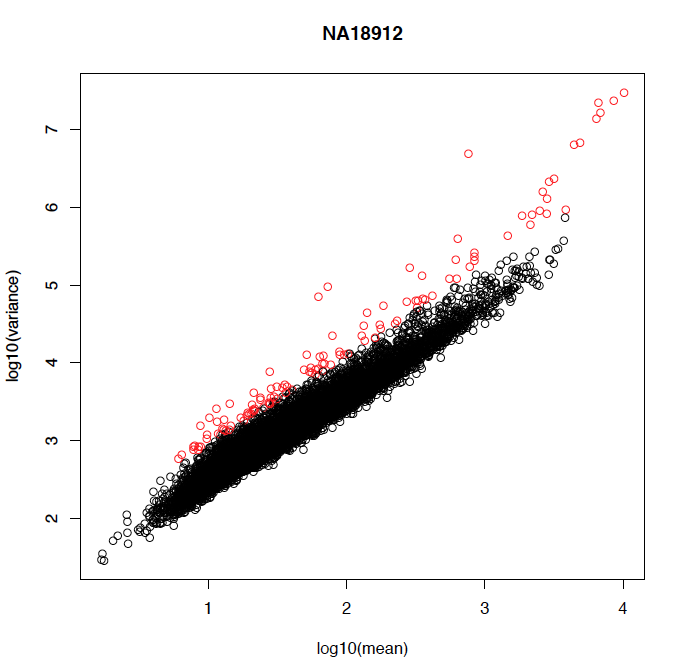
\includegraphics[width=\linewidth, scale=0.5]{figures/intro/intro_outlier1.png}
    \caption[SARGENT measures the insertion effect of a transgene.]{%
        \textbf{SARGENT measures the insertion effect of a transgene.}
        \subref{fig:cas_figure6a}
        Schematic for expression change detection in the transcriptome data.
     
    }
    \label{fig:outliervariance}
\end{figure}


Francesca et al. used 10X scRNA-seq data from X sampels and attempted to find QTLs. They found. 


- Talk about Yoav's paper. The search for variance QTLs. Francesca's paper

\subsubsection{Selection on noise levels}

\subsubsection{Noise in transcription factors}
It remains to be well understood how the noise in the upstream regulators of a pathway propagates through a pathway. Chang et al. \cite {sui_huang} showed that the variation in the transcription factor can have an effect on which way a cell differentiates.


Genetically identical yeast when grown in the same environment express different amounts of the same
protein. The stochasticity is due to biochemical fluctuations in the small number of molecules involved in
gene expression. In this Aim, I will address the question of whether the observed variability in the expression
of a gene is shared with other genes in the genome. Most studies of gene expression stochasticity have focused
on one locus or a few loci with a synthetic or endogenous gene. These studies have established that most
of the variance at a locus is due to cell-to-cell variability4. However, it is not known if cells with different
amounts of a protein are in different cell-states. Aim1 will address these questions.

We looked at the fluctuations in the transcriptionf actor 





%figure1
\begin{figure}[t!]  
    \centering
    \phantomlabel{fig:cas_figure6a}
    \phantomlabel{fig:cas_figure6b}
    \phantomlabel{fig:cas_figure6c}
    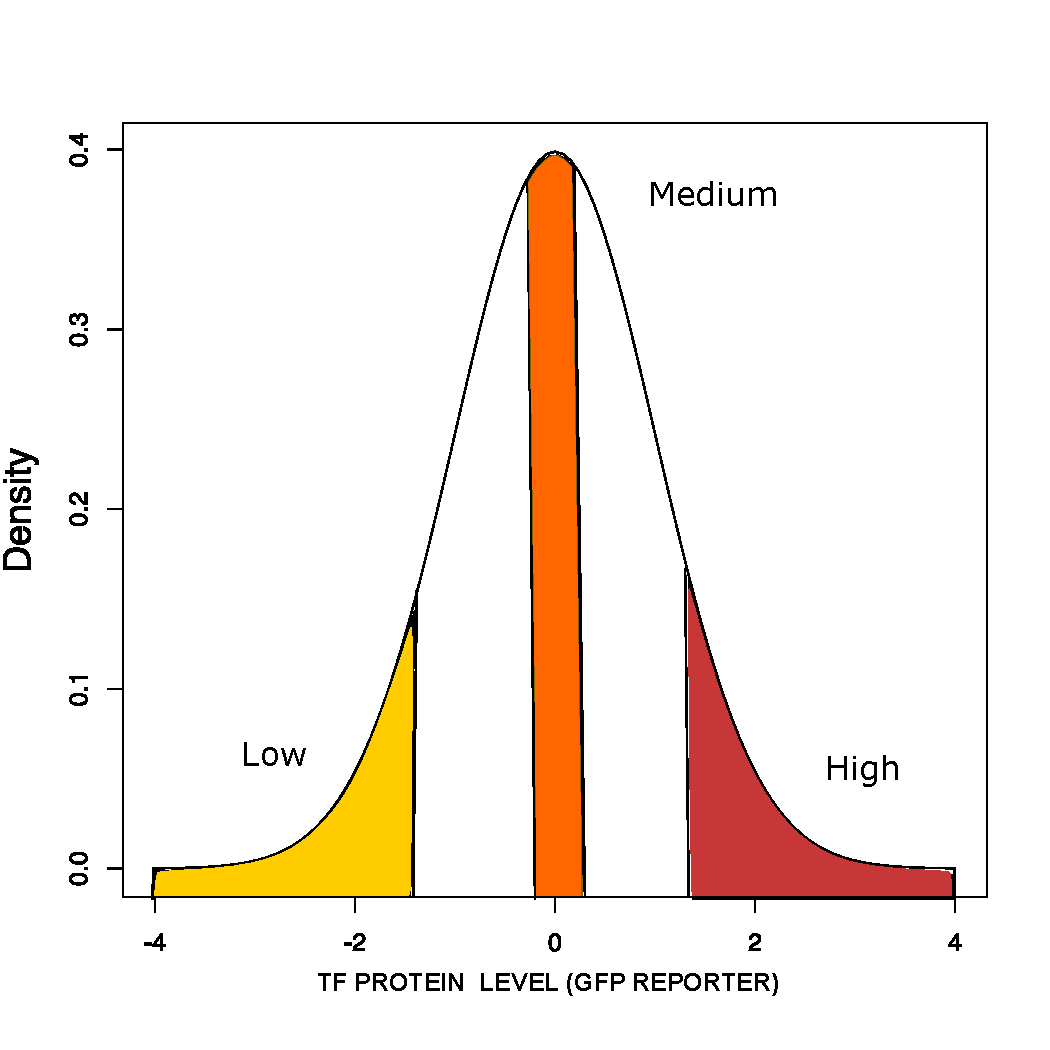
\includegraphics[width=\linewidth, scale=0.5]{figures/intro/intro_gfp_density_X.pdf}
    \caption[SARGENT measures the insertion effect of a transgene.]{%
        \textbf{SARGENT measures the insertion effect of a transgene.}
        \subref{fig:cas_figure6a}
        Schematic for expression change detection in the transcriptome data.
     
    }
    \label{fig:gfpXdensity}
\end{figure}



%figure1
\begin{figure}[t!]  
    \centering
    \phantomlabel{fig:cas_figure6a}
    \phantomlabel{fig:cas_figure6b}
    \phantomlabel{fig:cas_figure6c}
    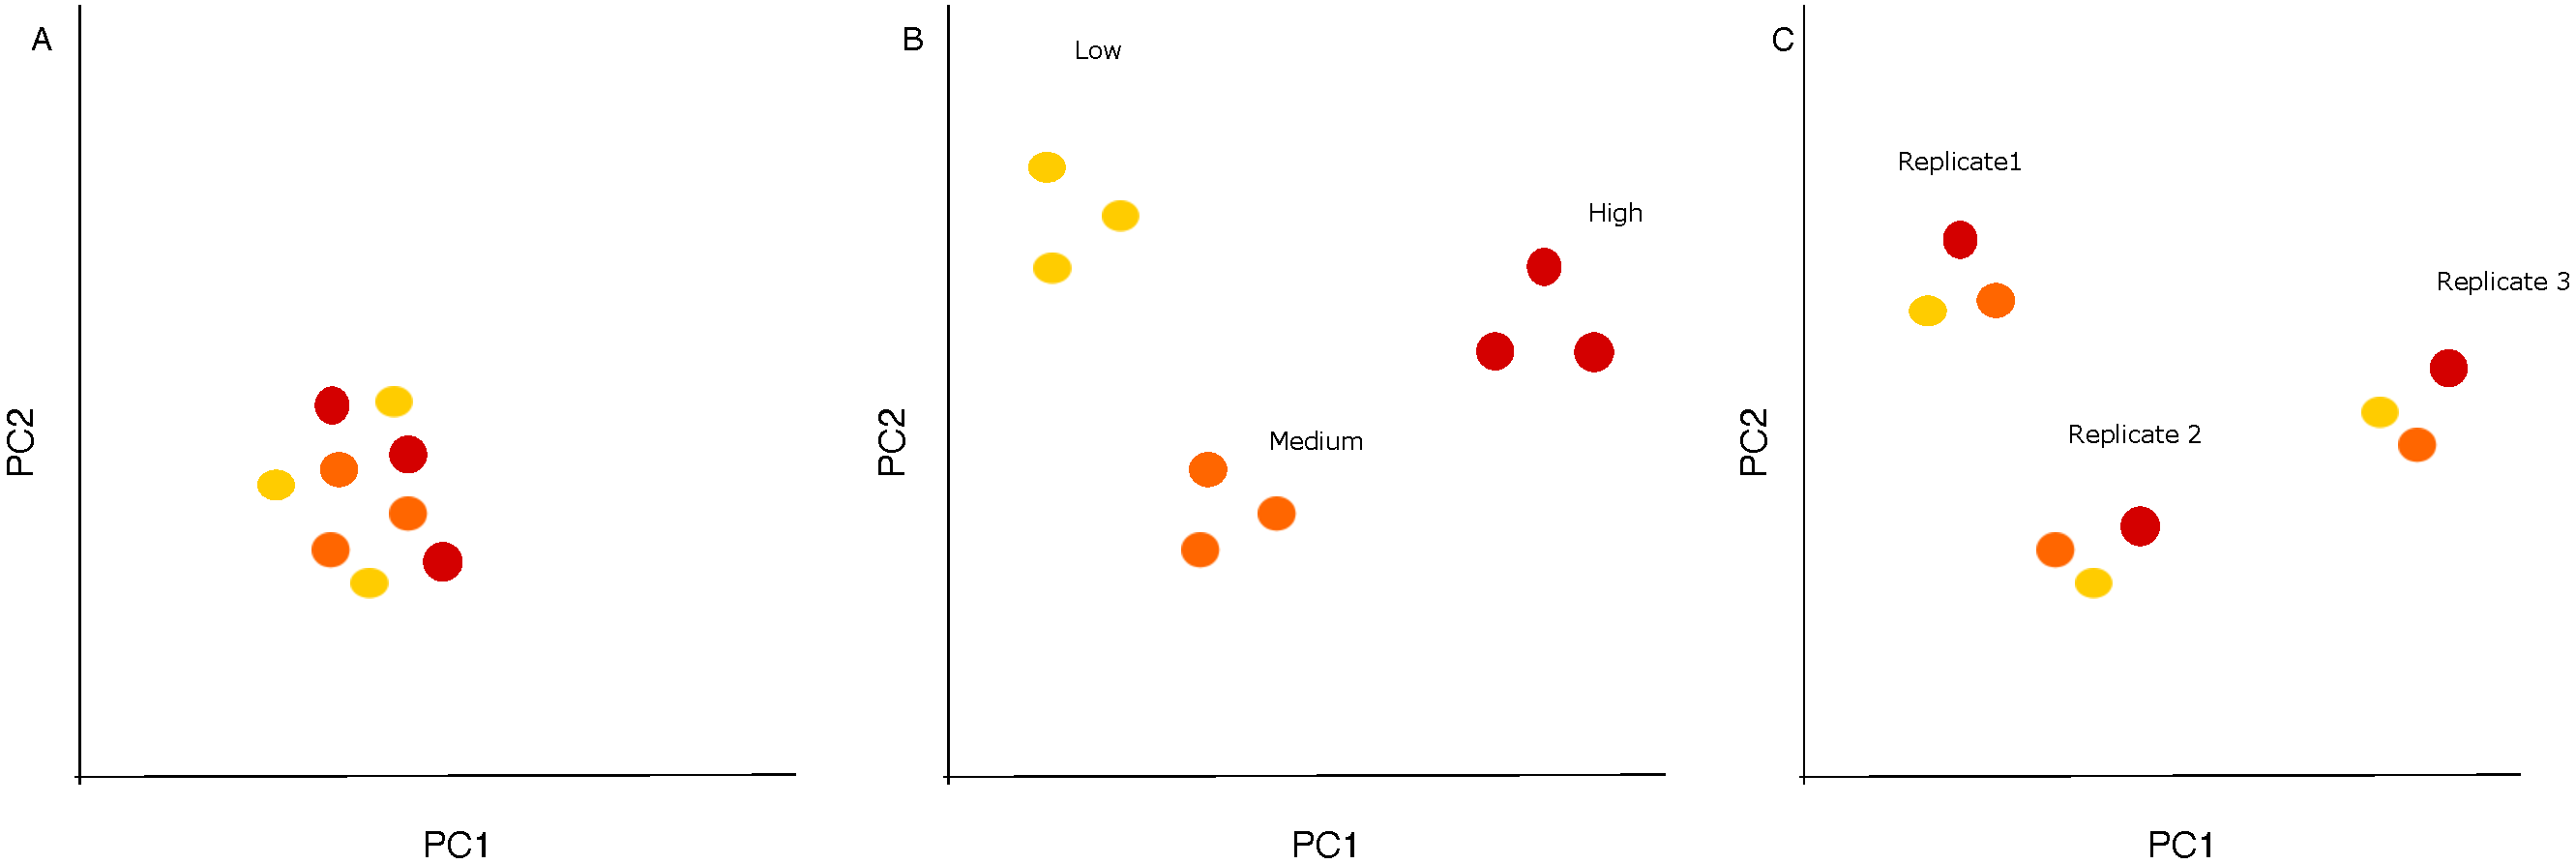
\includegraphics[width=\linewidth, scale=0.5]{figures/intro/intro_aim1_task1.pdf}
    \caption[SARGENT measures the insertion effect of a transgene.]{%
        \textbf{SARGENT measures the insertion effect of a transgene.}
        \subref{fig:cas_figure6a}
        Schematic for expression change detection in the transcriptome data.
     
    }
    \label{fig:aim1_task1}
\end{figure}



%figure1
\begin{figure}[t!]  
    \centering
    \phantomlabel{fig:cas_figure6a}
    \phantomlabel{fig:cas_figure6b}
    \phantomlabel{fig:cas_figure6c}
    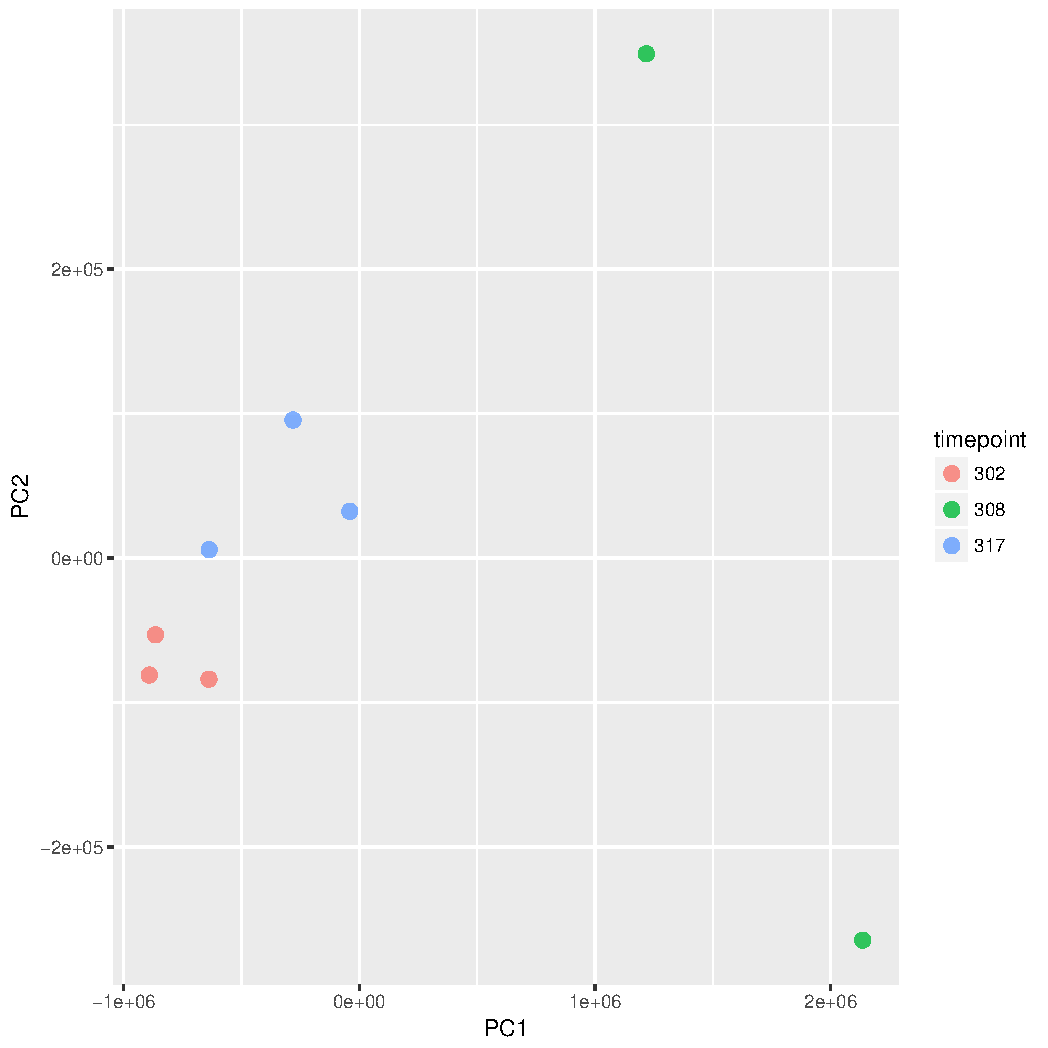
\includegraphics[width=\linewidth]{figures/intro/intro_tdh2_pca.pdf}
    \caption[SARGENT measures the insertion effect of a transgene.]{%
        \textbf{SARGENT measures the insertion effect of a transgene.}
        \subref{fig:cas_figure6a}
        Schematic for expression change detection in the transcriptome data.
     
    }
    \label{fig:tdh2_pca}
\end{figure}
\subsubsection{Effect of chromatin on mean and noise}
\subsubsection{Effect of sequence features on noise}

\subsection{ Is teh variability shared betwen pathway members}
Talk about your TDH3 results here. Also setup for the cell-state story of CAS.

\subsection{Scope of thesis work}
This thesis consists of two main works.

In  Chapter 2 I will try to explain the sources of variability observed within a cell-type. I will test the hypothesis that cells of the same cell-type express different subsets of genes due to stochastic activation of upstream regulators. Specifically, I will test the hypothesis that stochastic expression of transcription factors and stochastic activation of signaling pathways leads to variability between cells of the same cell-type.

In Chapter 3, I aim to understand what determines the noise levels of different genes in the genome. In collaboration with two other graduate students I devised a new genomic technology called SARGENT (Single-cell Analysis of Reporter Gene Expression Noise and Transcriptome) to study noise genome-wide. Using SARGENT, we integrats the same reporter gene in multiple genomic locations and measure the cell-to-cell variability in expression of this reporter gene using single-cell RNA sequencing. We then attempt to understand the determinants of this noise, after removing the effect of the mean level of expression, using the chromatin state and sequence features at different genomic locations. We also decompose the variability into extrinsic and intrinsic noise, and understand the determinants of these two noise sources. SARGENT also allows us to identify cell-states and quantify the impact of cell-states on noise.
